To get a clearer picture of the data, we will first make a loose cut selecting only events with $\chi^2_\nu < 10$. We can then generate phase-space Monte Carlo for the $4\pi$ background reaction and search for potential ways to separate it from the signal by comparing the distributions of common kinematic variables.

\begin{figure}
  \begin{center}
    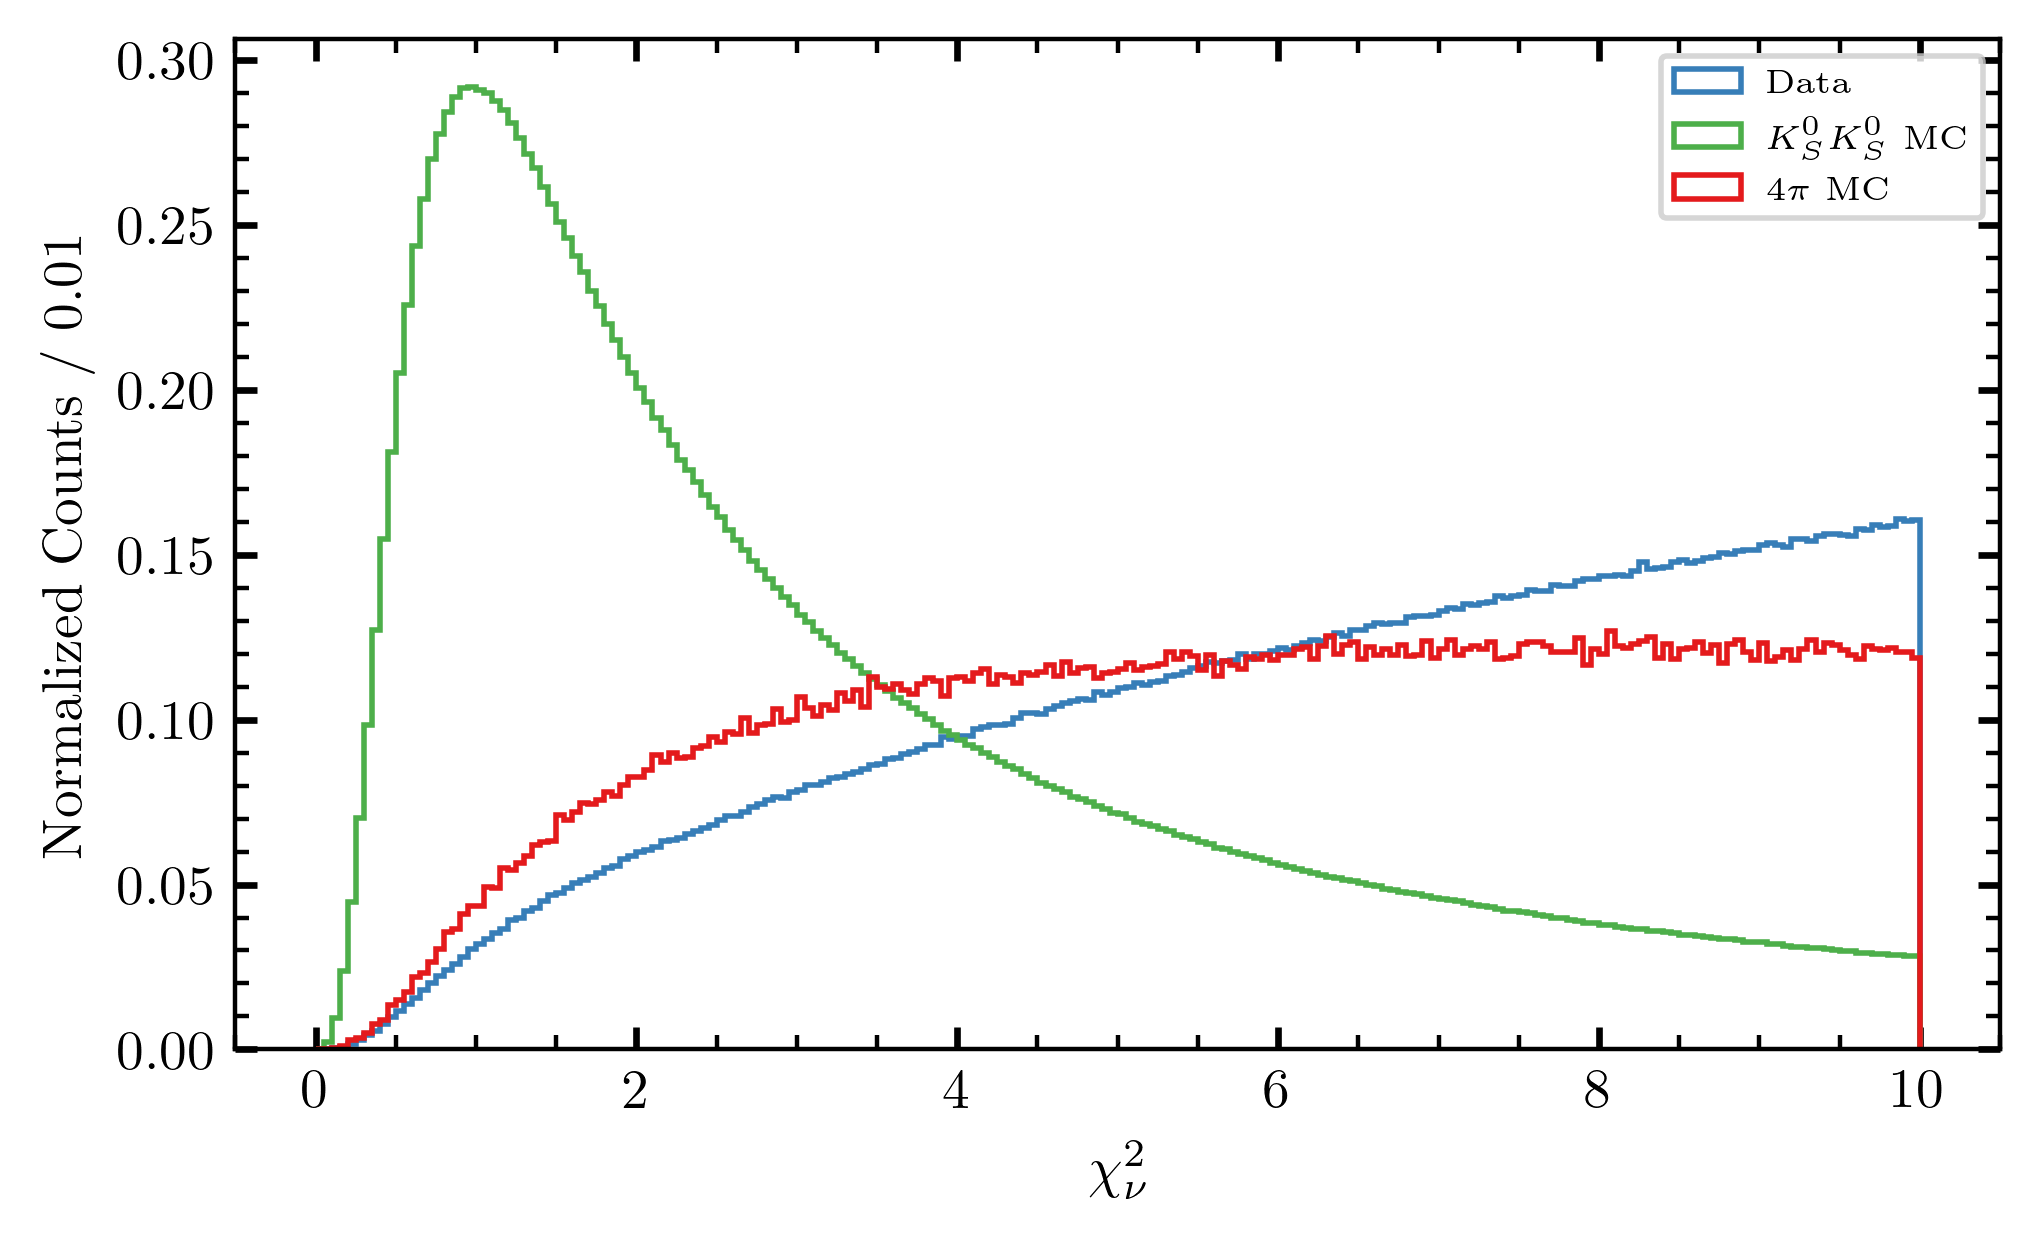
\includegraphics[width=0.8\textwidth]{figures/data_combined_chisqdof.png}
  \end{center}
  \caption{The normalized distributions of $\chi^2_\nu$ for the true data and phase-space signal and $4\pi$ background Monte Carlo.}\label{fig:data-combined-chisqdof}
\end{figure}

In \Cref{fig:data-combined-chisqdof}, we can see the various distributions of the data and each simulated channel. Unfortunately, the data distribution resembles the $4\pi$ background distribution much better than the signal Monte Carlo, but now we also know that the signal decays rapidly at higher values of $\chi^2_\nu$, so a tighter selection might improve the signal-to-background ratio, even if we cannot immediately see a peak in the data near unity. We can use the overall probability densities from the Monte Carlo simulations to inform our decision on where to place a cut. We begin by defining the true/false positive rates as

\begin{align}
  \epsilon_S(\chi^{2*}_\nu) &= \int_0^{\chi^{2*}_\nu} \dd{(\chi^2_\nu)} p_S(\chi^2_\nu) \\
  \epsilon_B(\chi^{2*}_\nu) &= \int_0^{\chi^{2*}_\nu} \dd{(\chi^2_\nu)} p_B(\chi^2_\nu),
\end{align}
where $p_S(\chi^2_\nu)$ and $p_B(\chi^2_\nu)$ are the probability densities of the signal and background Monte Carlo, respectively, calculated from the normalized distributions over $\chi^2_\nu$ detailed in \Cref{fig:data-combined-chisqdof}. The Youden J-statistic~\cite{Peirce1884,Youden1950} can be used as a criterion for finding the optimal cut value $x_c$~\cite{Schisterman2005,Powers2020}. It relates the sensitivity ($\epsilon_S$) and the specificity ($1-\epsilon_B$) as

\begin{equation}
  J(\chi^{2*}_\nu) = \epsilon_S(\chi^{2*}_\nu) - \epsilon_B(\chi^{2*}_\nu).
  \label{eq:youden-j}
\end{equation}

The Youden J-index is equivalent to the distance between the no-discrimination line and the receiver operating characteristic (ROC) curve shown in \Cref{fig:data-combined-chisqdof-roc}. The index itself as a function of cut value is shown in \Cref{fig:data-combined-chisqdof-youden-j}, and it is maximized at a cut value of $\chi^{2*}_\nu = 3.4$. This indicates the boundary where we can make a maximally informed decision between labels of signal and background for each event. It is not equivalent to some measure of signal purity, since it makes no use of the relative proportion of signal to background in the data. Because our data is clearly background dominated, a requirement of high signal purity would lead to very low overall statistics, and we still have other methods of separating signal from background which will allow us to improve the signal-to-background ratio without dramatic cuts on the total number of signal events (see \Cref{sec:splot}). The given cut maximizes the net improvement over random guessing, and as it does not assume a prior on the signal-to-background ratio, it is a good starting point which we can adjust later depending on how much background we wish to remove. We will analyze the effect of using a different value for this cut in \Cref{sec:systematic-studies}.

\begin{figure}
  \begin{center}
    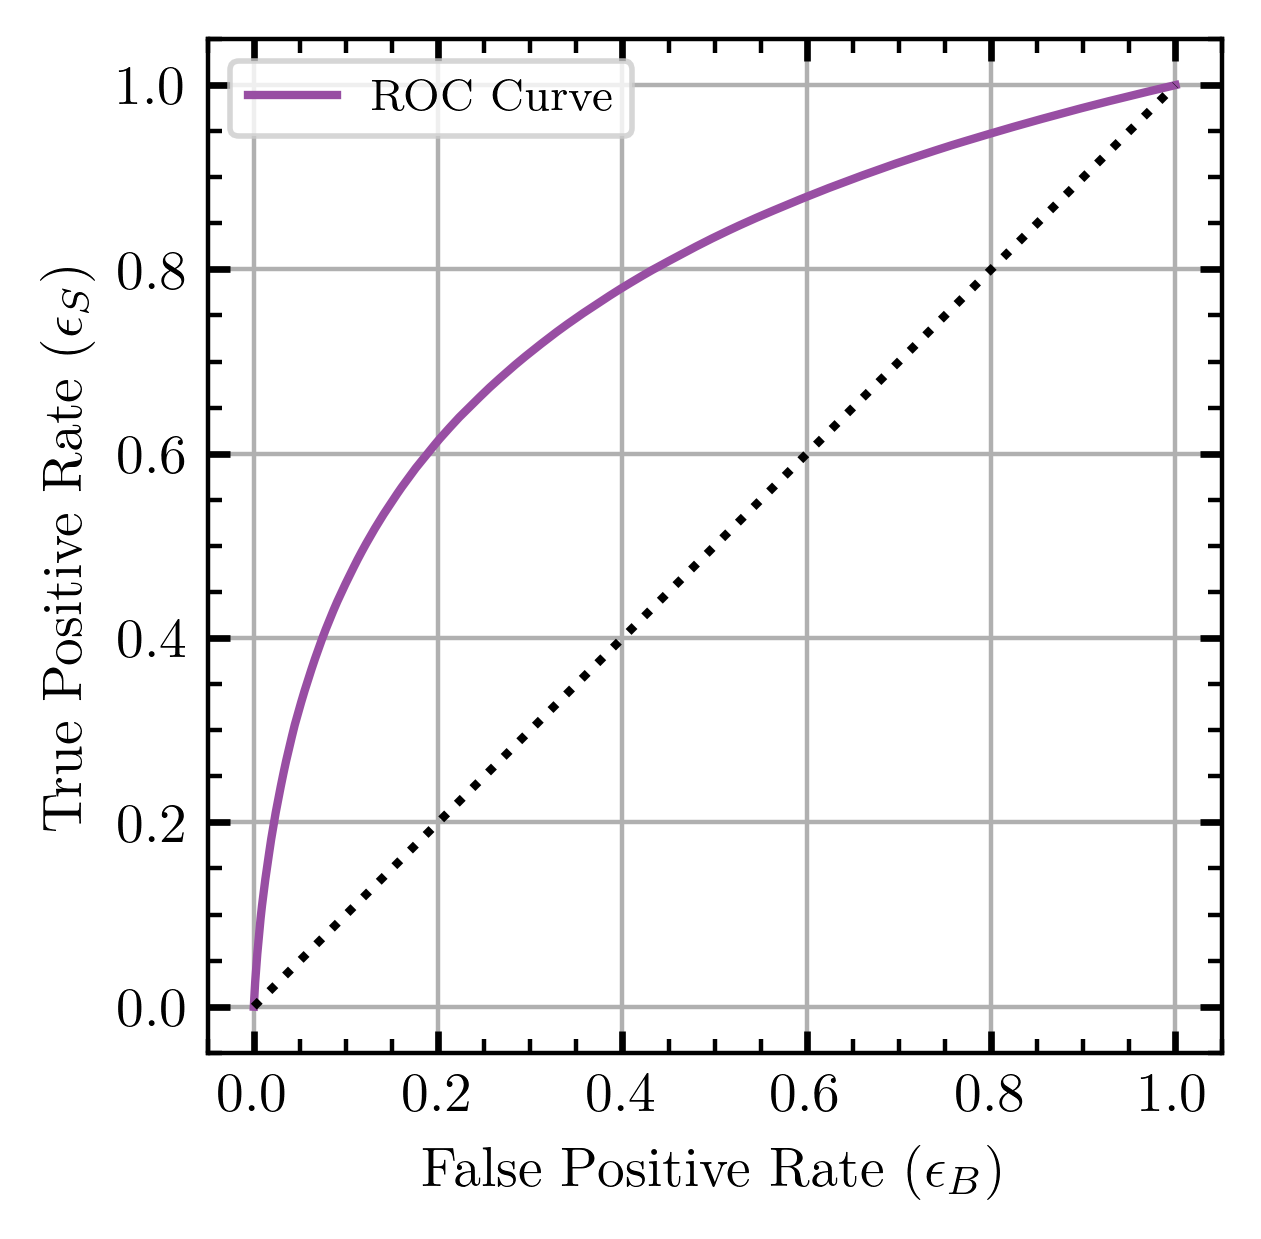
\includegraphics[width=0.8\textwidth]{figures/data_combined_chisqdof_roc.png}
  \end{center}
  \caption{The receiver operating characteristic (ROC) curve for selections on $\chi^2_\nu$ constructed from the signal and background Monte Carlo distributions.}\label{fig:data-combined-chisqdof-roc}
\end{figure}

\begin{figure}
  \begin{center}
    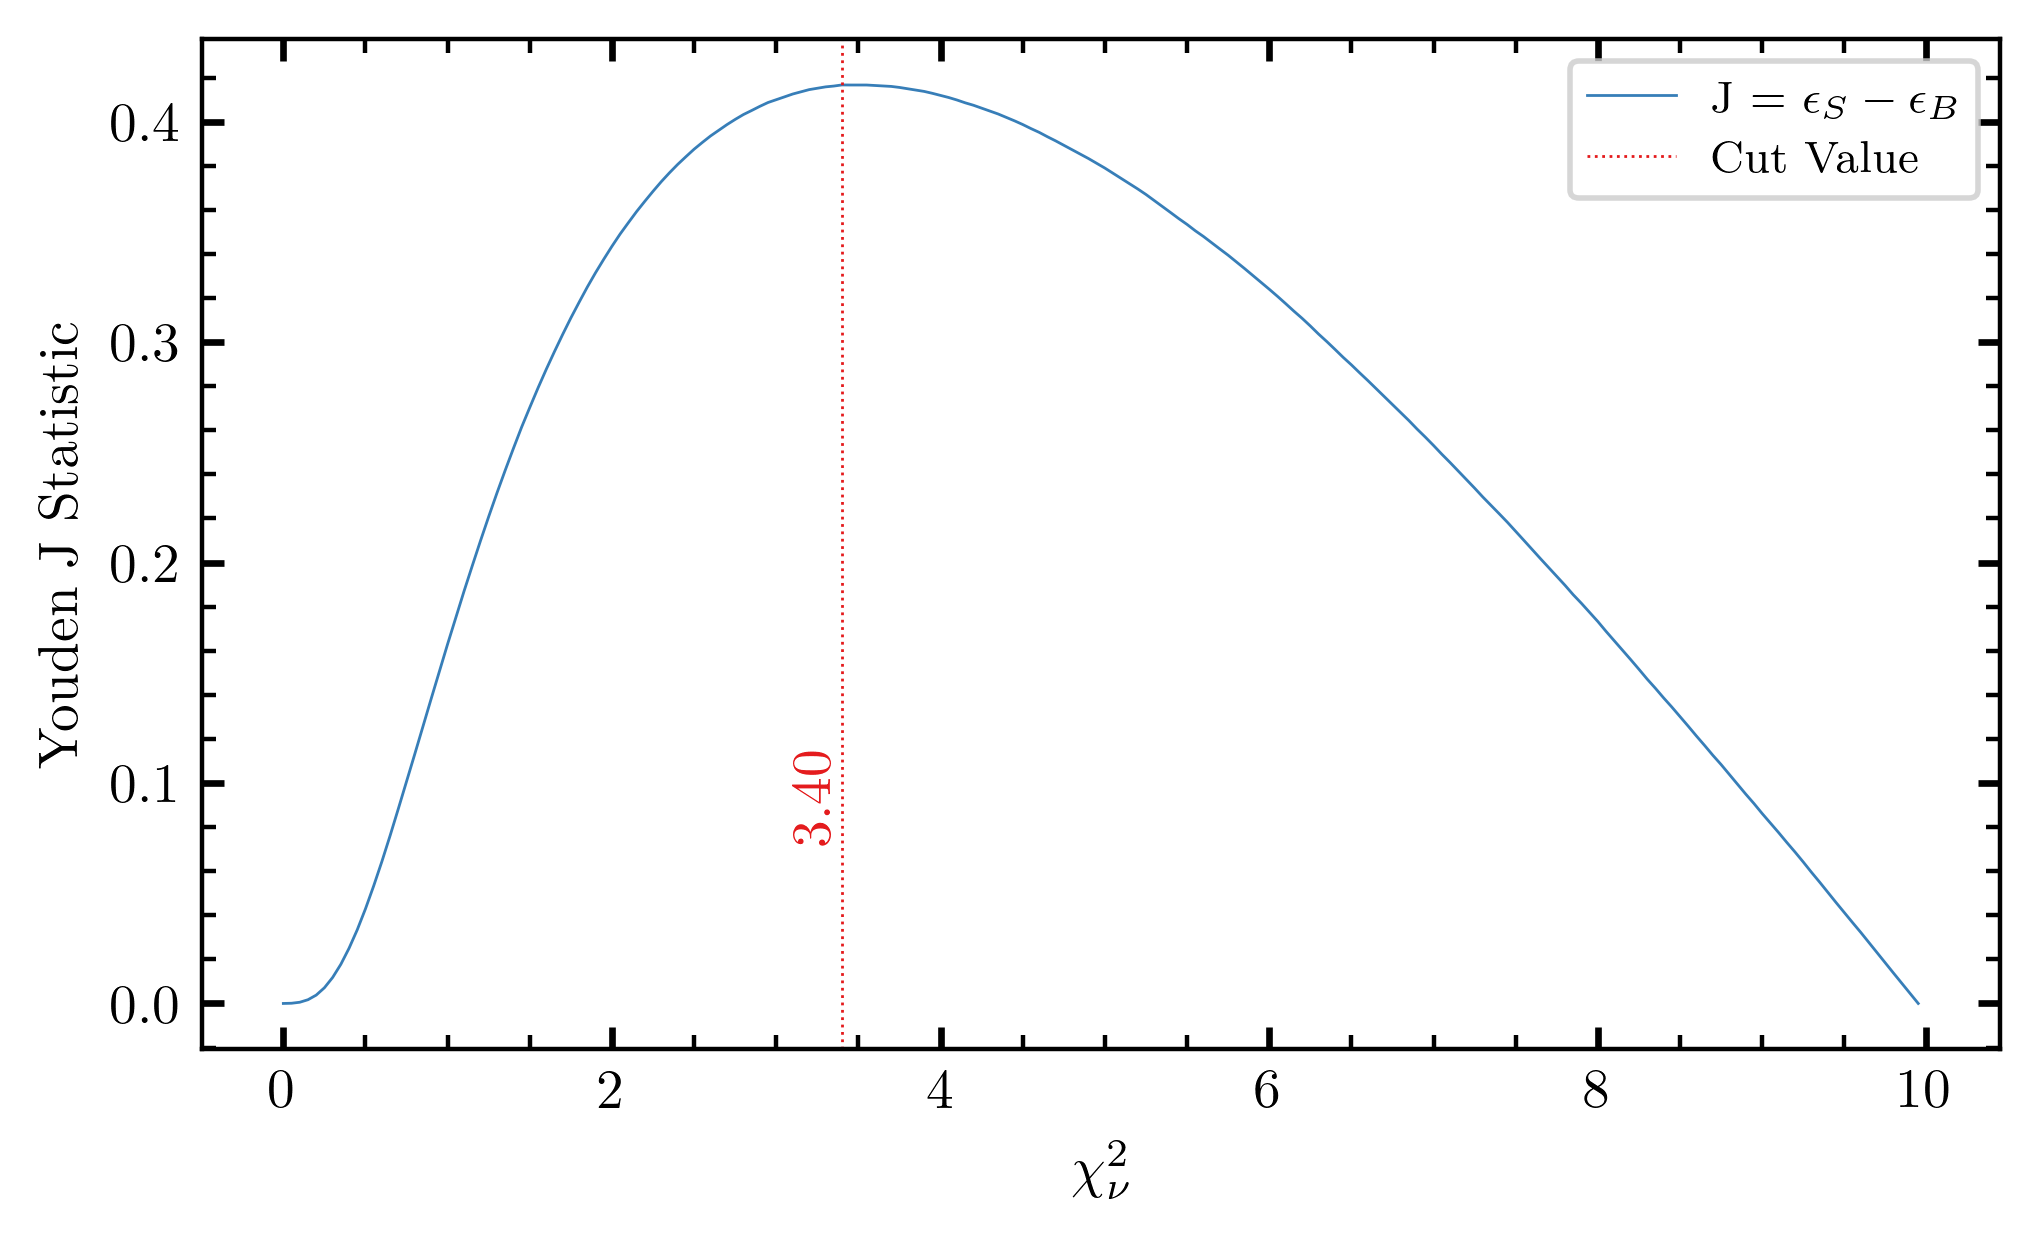
\includegraphics[width=0.8\textwidth]{figures/data_combined_chisqdof_youden_j.png}
  \end{center}
  \caption{The Youden J-statistic for selections on $\chi^2_\nu$ constructed from the signal and background Monte Carlo distributions. The maximal value indicates a selection at $\chi^2_\nu = 3.4$ would be the maximally informed decision boundary.}\label{fig:data-combined-chisqdof-youden-j}
\end{figure}


\begin{figure}
  \begin{center}
    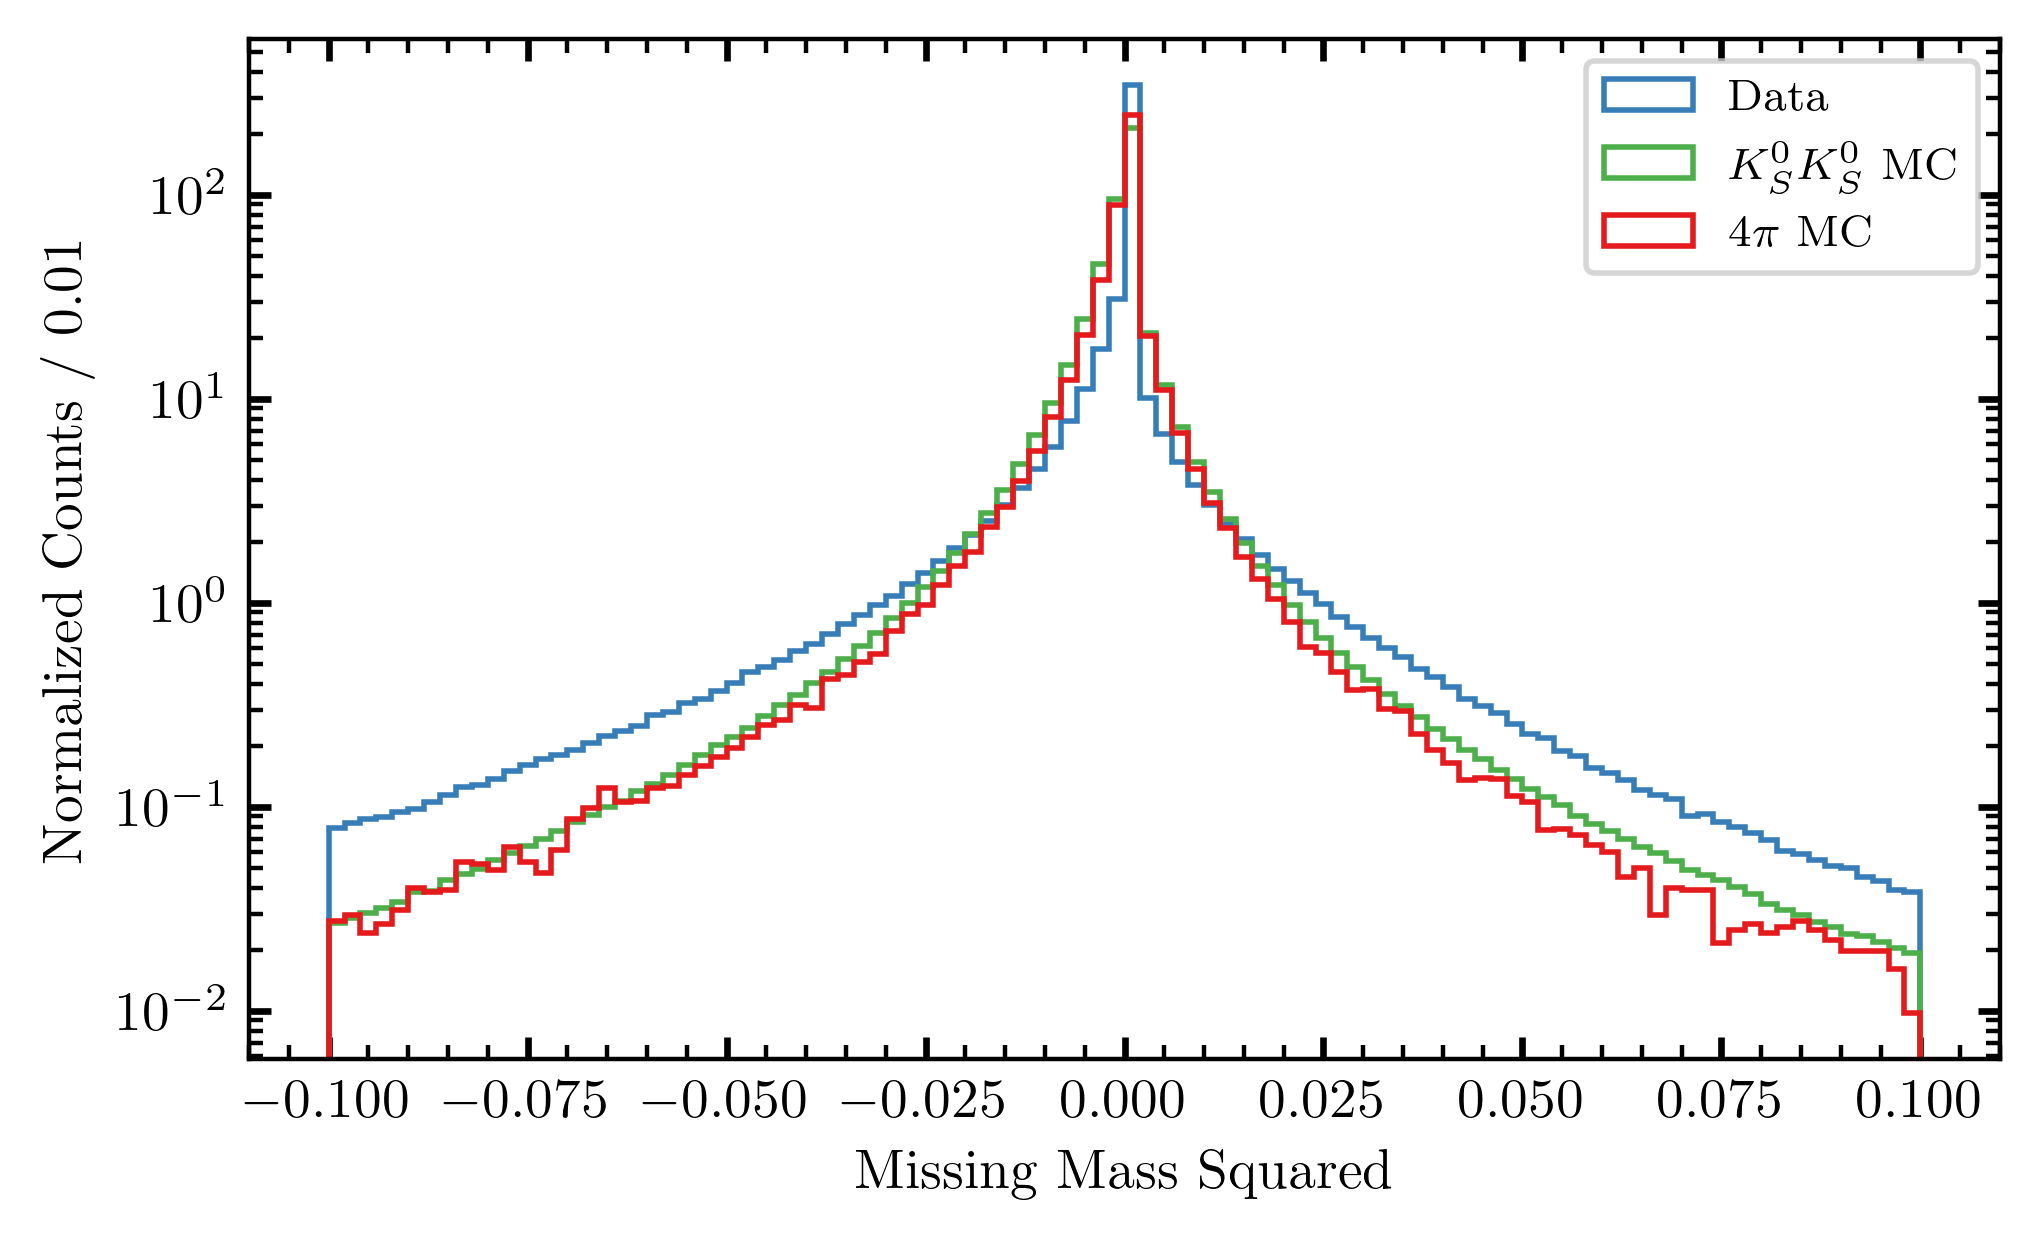
\includegraphics[width=0.8\textwidth]{figures/data_combined_mm2.png}
  \end{center}
  \caption{The normalized distributions of missing mass squared for the true data and phase-space signal and $4\pi$ background Monte Carlo.}\label{fig:data-combined-mm2}
\end{figure}

Another common selection which can be made is on the squared missing mass of an event, which is just the square of the difference between the initial- and final-state four-momenta. This variable, visualized in \Cref{fig:data-combined-mm2}, predictably peaks at zero for the data, signal Monte Carlo, and background Monte Carlo, and the overall distributions for the signal and backgound simulated events are nearly identical. This indicates that a selection on this variable would not be very useful at distinguishing the signal from the background.

Recall that the main difference between the signal and background channels described here is the presence of decaying $K_S^0$ particles in the signal channel. These particles have a well-known lifetime around $\SI{89.54}{\pico\second}$ due to their decay into non-strange mesons requiring a weak interaction. While we might not know the exact process which creates the $4\pi$ background, we can assume a strong interaction produces the pions, which should happen several orders of magnitude faster than the $K_S^0$ decay. Due to the resolution of the detector, we still expect these events to appear to have some non-zero distribution in rest-frame lifetime when we mistakenly interpret pairs of pions as kaons, but it will be vastly different from that of the signal.

\begin{figure}
  \begin{center}
    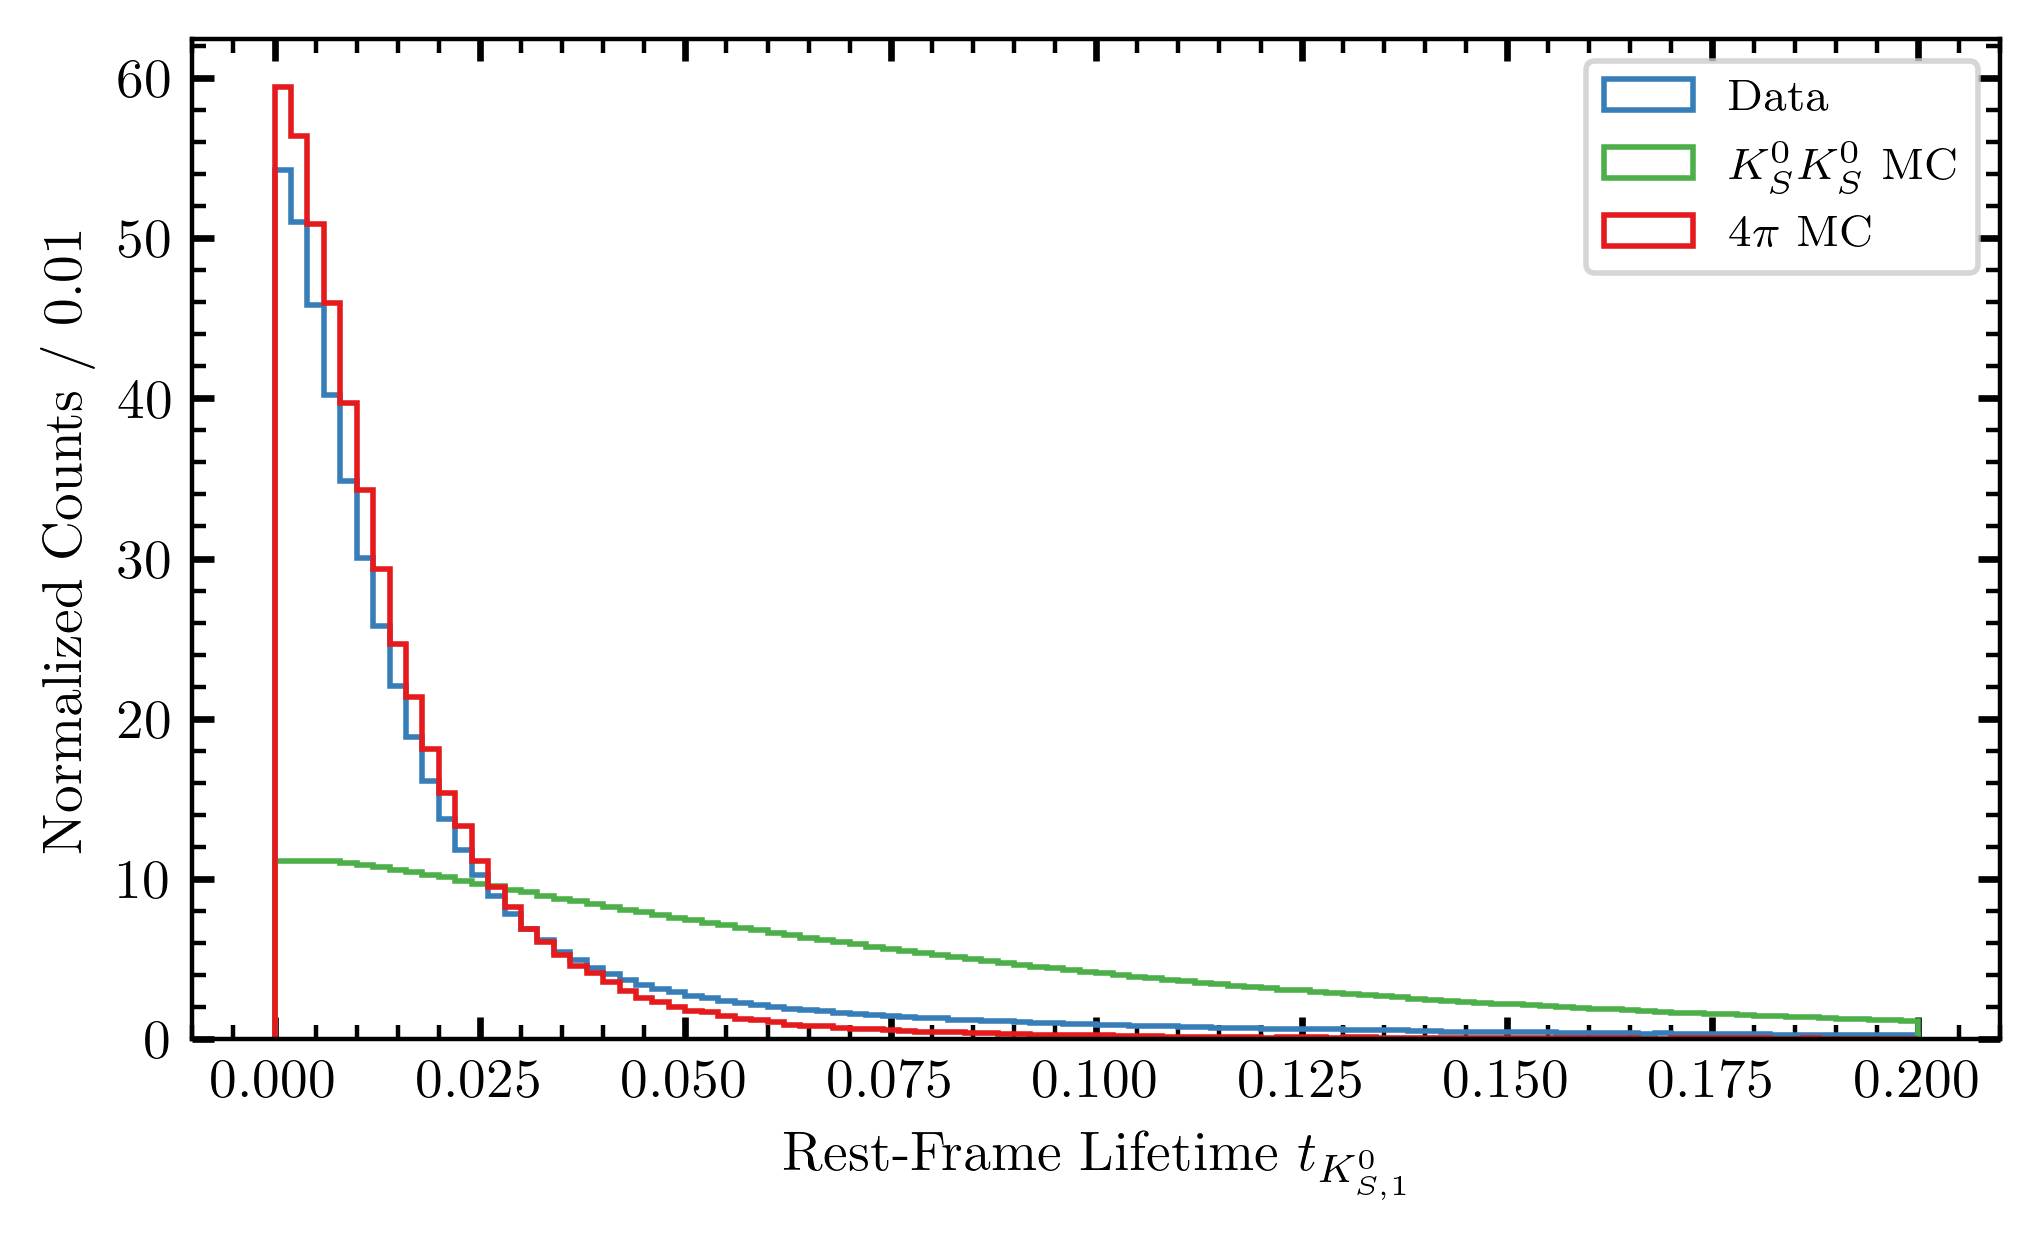
\includegraphics[width=0.8\textwidth]{figures/data_combined_rfl.png}
  \end{center}
  \caption{The normalized distributions of the rest-frame lifetime of one of the $K_S^0$ candidates for the true data and phase-space signal and $4\pi$ background Monte Carlo.}\label{fig:data-combined-rfl}
\end{figure}

We can see the effect of this in \Cref{fig:data-combined-rfl}. The exponential slope of the signal Monte Carlo is distinct from that of the background Monte Carlo, but the data distribution is dominated by this background. While we could use the Youden J-statistic again to determine a cut, the largest portion of the true signal appears in the same place as the largest portion of background, and we would have to remove many good events just to get rid of the majority of the background. Rather than performing a hard cut on rest-frame lifetime, we will instead use statistical weighting methods described in \Cref{sec:splot}.

Before we do this, however, there is one more minor selection which we will perform, which is a selection on the $z$-vertex of the target proton. We know the exact location of the target with respect to the detector, and we only want to deal with events which we know originated inside this target. The distribution of the $z$-vertex values can be seen in \Cref{fig:data-original-combined-protonz}. We will select events with $\SI{50}{\centi\meter} < z < \SI{80}{\centi\meter}$, as this is the known length and position of the target relative to the detector elements. While there is an indication of events in the signal Monte Carlo in the regions which are removed, we know that while these events originated from the target, their $z$-vertex has been misidentified, so we should remove them anyway.


\begin{figure}
  \begin{center}
    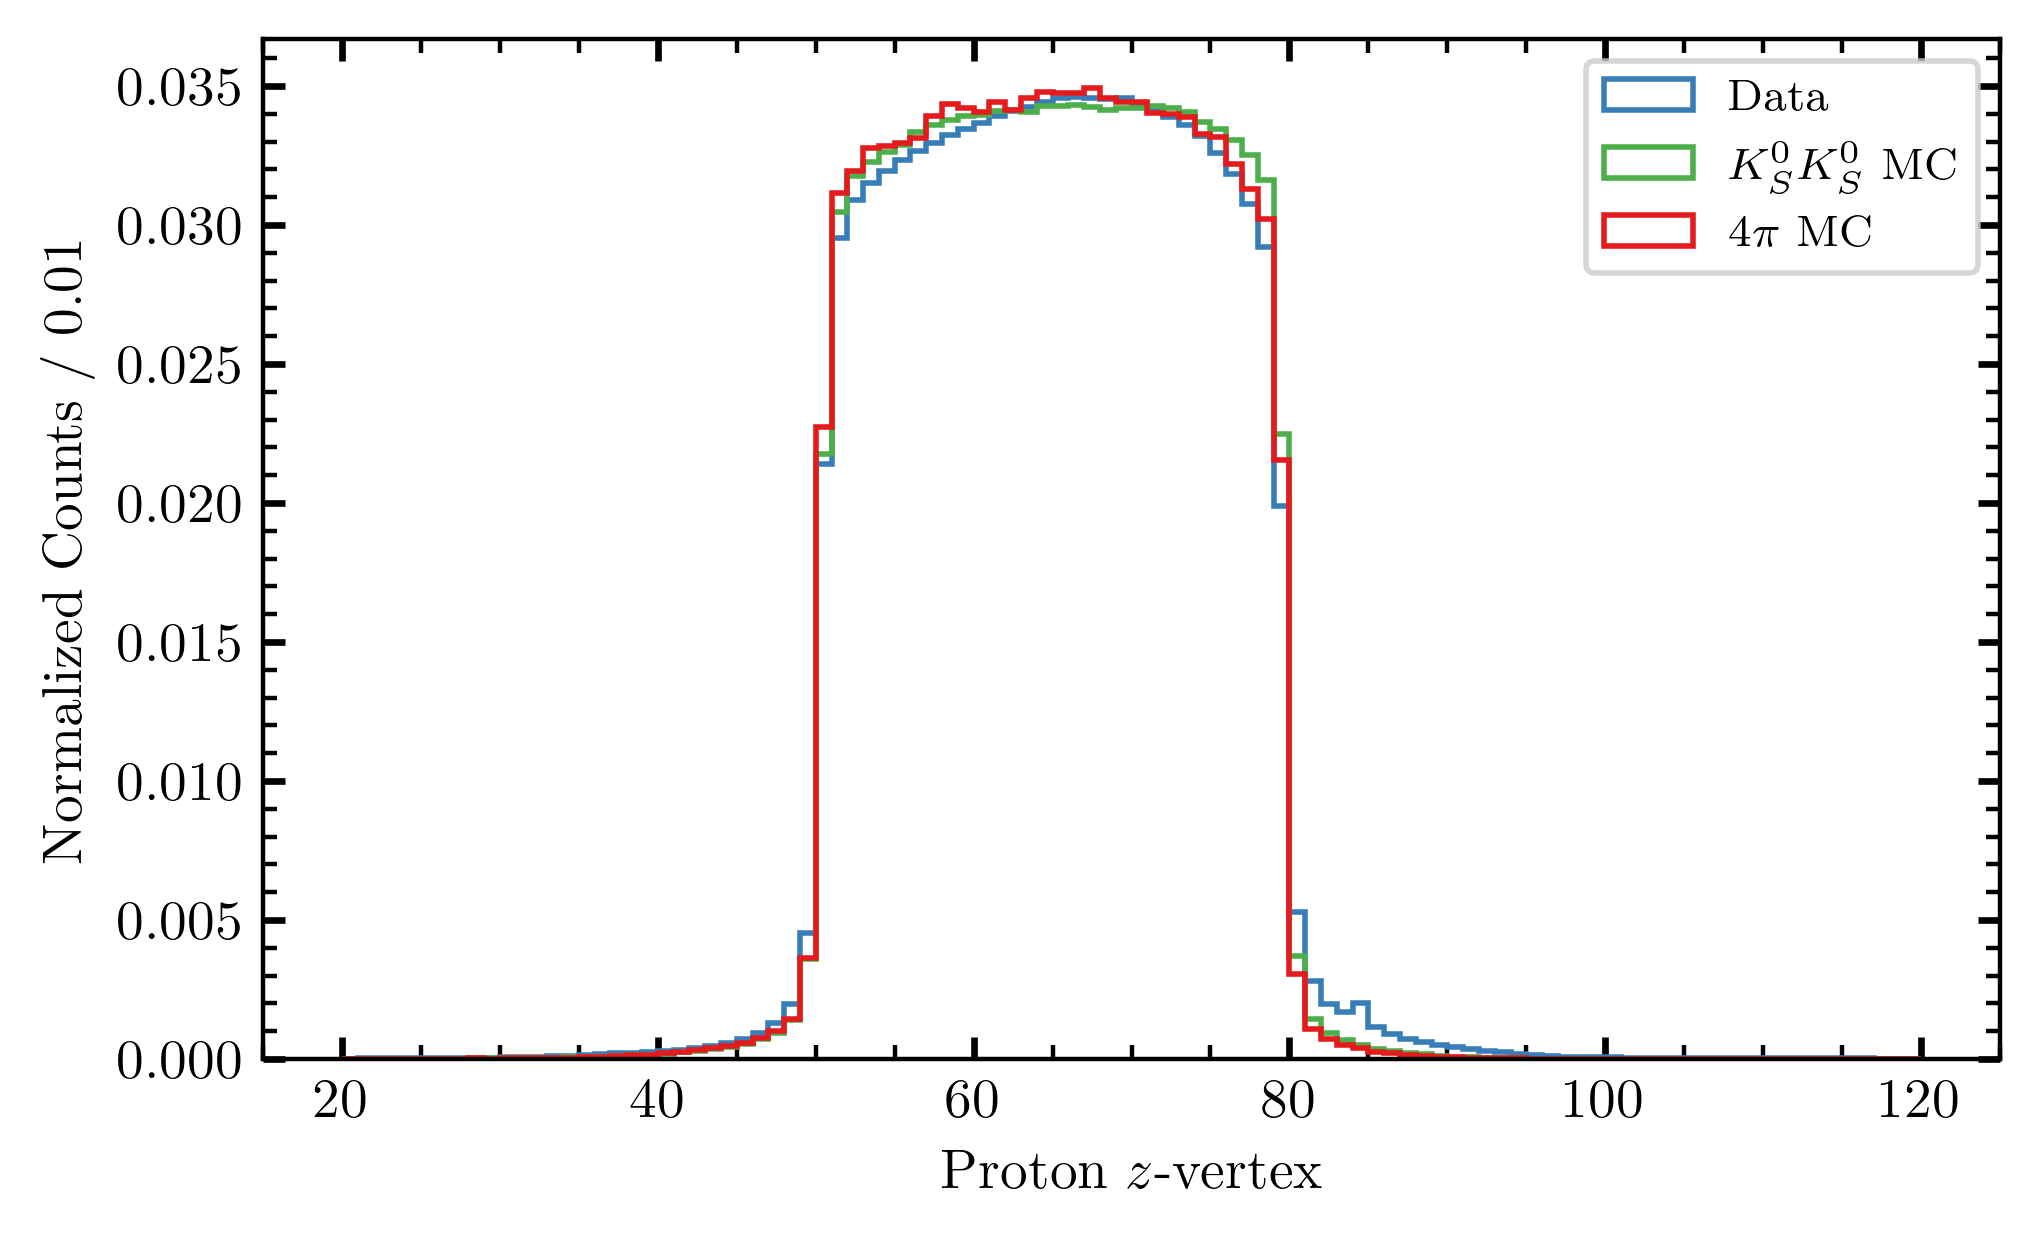
\includegraphics[width=0.8\textwidth]{figures/data_original_combined_protonz.png}
  \end{center}
  \caption{The normalized distributions of the target proton $z$-vertex for the true data and phase-space signal and $4\pi$ background Monte Carlo.}\label{fig:data-original-combined-protonz}
\end{figure}

{\color{red}TODO: dE/dx plots in CDC, FDC for $p$/$\pi$ separation (appendix?)}

The impetus for studying this channel was originally a search for excited hyperons\textemdash baryons with strange quark content. In particular, $\Sigma^+$ resonances should form in the invariant mass distribution of $K_S^0 p$, where the other kaon is required to conserve strangeness in the strong production of this baryon. After the cuts mentioned above, the spectrum of these $\Sigma^+$ resonances is shown in {\color{red}TODO FIGURE}. However, there is a symmetry between the identical kaons which must be accounted for. We could pair either kaon with the proton to form the $\Sigma^+$, but there is a more likely pairing which can be found by first assuming that the heavier hyperon will generally move more backwards in the center-of-momentum frame than the lighter bachelor $K_S^0$. Therefore, the kaon which is moving in a further backward direction is more likely to correspond with the hyperon decay candidate. We can sort the kaons by their $\cos\theta$ in the center-of-momentum frame and call the more backward-going kaon $K_{S,B}^0$. The invariant mass spectrum of $K_{S,B}^0 p$ can be seen in {\color{red}TODO FIGURE}. The enhancement around $\SI{1.7}{\giga\electronvolt}$ likely corresponds to some combination of the $\Sigma^+(1660)$, $\Sigma^+(1670)$, $\Sigma^+(1750)$, and $\Sigma^+(1775)$ resonances. We do not see much indication of states above $\SI{2}{\giga\electronvolt}$.

This angle also gives us a handle on separating baryonic and mesonic topologies. If we plot the $\cos\theta$ of $K_{S,B}^0$ against the invariant mass of $K_{S,B}^0 p$, as in {\color{red}TODO FIGURE}, we find a strong and somewhat expected dependence. The majority of the baryonic contribution occurs at angles with $\cos\theta < 0$. Likewise, the mesonic contribution is mostly confined to angles of $\cos\theta > 0$, as seen in figures {\color{red}TODO ksks mass and mass vs angle}. While it may not be obvious that there even are meson resonances here, we will see their contributions much more clearly after the statistical weighting procedures defined in \Cref{sec:splot} have been applied, after which we will revisit these plots. We will also conduct our analysis without this selection in \Cref{sec:systematic-studies} for completeness.

In total, we only have three main fiducial selections on the data, as illustrated in \Cref{tab:fiducial-cuts}.

\begin{table}
  \begin{center}
    \begin{tabular}{cc}\toprule
      Variable & Selected Values \\\midrule
      $\chi^2_\nu$ & $\chi^2_\nu < 3.4$ \\
      Target proton-$z$ & $\SI{50}{\centi\meter} < z < \SI{80}{\centi\meter}$ \\\bottomrule
      $\cos\theta_{\text{CM}}$ of $K_{S,B}^0$ & $ \cos\theta_{\text{CM}} > 0.0 $
    \end{tabular}
    \caption{Fiducial cuts performed after event reconstruction.}\label{tab:fiducial-cuts}
  \end{center}
\end{table}
